\chapter{Literature Review}
% Main Gist 
% - History of FHR reactor type and why there is a renewed interest in this
%   reactor type (start ups, labs etc.)
% - Past applications of AI to nuclear reactor design. 
% Structure 
% - Fluoride-Salt-Cooled High-Temperature Reactor (why salt cooled triso fuelled 
%   reactors are cool)
%   - FHR Modeling Challenges (why benchmark exists)
%   - Description of benchmark
% - Artificial Intelligence Applications to Nuclear Reactor Design Optimization
%   - Past work 
%   - Classical vs Evolutionary methods 

\section{Fluoride-Salt-Cooled High-Temperature Reactor}
The \gls{FHR} is a reactor concept introduced in 2012 that uses high-temperature 
coated-particle fuel and a low pressure liquid fluoride-salt coolant 
\cite{forsberg_fluoride-salt-cooled_2012,facilitators_fluoride-salt-cooled_2013}.
\gls{FHR} technology combines the best aspects of \gls{MSR} and \gls{VHTR} 
(or \gls{HTGR}) technologies. 
Molten fluoride salts as working fluids for nuclear reactors have been explored 
since the 1960s and are desirable because of the salts' high-temperature 
performance and overall chemical stability \cite{scarlat_design_2014}.  
Using molten salts for reactor coolant introduces inherent safety compared 
to water due to the salts' high boiling temperature and high volumetric 
heat capacity, eliminating the risk of coolant boiling off, resulting in 
fuel elements overheating \cite{ho_molten_2013}. 
The leading candidate coolant salt is the fluoride salt Li$_2$BeF$_4$ (FLiBe), 
which remains liquid without pressurization up to 1400 $^{\circ}$C and a larger 
$\rho C_p$ than water \cite{ho_molten_2013,forsberg_fluoride-salt-cooled_2012}. 
\glspl{FHR} are favorable compared to a liquid fuel reactor, such as
\gls{MSR} systems, because the solid fuel cladding adds an extra barrier to fission 
product release 
\cite{ho_molten_2013}.

\gls{VHTR} technology has been studied since the 1970s because they delivers 
heat at substantially high temperatures than \glspl{LWR} resulting in 
the following advantages: increased power conversion efficiency, reduced 
waste heat generation, and co-generation and process heat capabilities 
\cite{scarlat_design_2014}. 
In \glspl{VHTR}, the helium coolant is held at a high pressure of approximately 
100 atm, whereas the \gls{FHR}'s FLiBe coolant is at room pressure, resulting in lower 
construction costs since a thick concrete reactor vessel is not required.
The molten salt coolant has superior cooling and moderating properties compared 
to helium coolant in \glspl{VHTR}, resulting in \glspl{FHR} operating at 
power densities two to six times higher than  \glspl{VHTR} 
\cite{scarlat_design_2014,forsberg_fluoride-salt-cooled_2012}.
Therefore, by combining the FLiBE coolant from \gls{MSR} technology and 
\gls{TRISO} particles from \gls{VHTR} technology, the \gls{FHR} benefits from 
the low operating pressure and large thermal margin provided by using a molten 
salt coolant and the accident-tolerant qualities of \gls{TRISO} particle fuel. 

There are several types of \gls{FHR} conceptual designs that exist
worldwide: \gls{PBFHR} at UCB with circulating pebble-fuel 
\cite{scarlat_current_2014,krumwiede_three-dimensional_2013}, the \gls{SF-TMSR} 
at the \gls{SINAP} in China with static pebble-fuel \cite{liu_preliminary_2016}, 
the large central-station \gls{AHTR} at \gls{ORNL} \cite{holcomb_core_2011, varma_ahtr_2012} and 
the \gls{SmAHTR} at ORNL \cite{greene_pre-conceptual_2010} with static plate-fuel. 

\subsection{AHTR design}
This proposed work is focused on the FHR design with hexagonal fuel elements 
consisting of \gls{TRISO} fuel particles embedded in plates ("planks"), i.e., the 
\gls{AHTR} design developed by ORNL. 
The \gls{AHTR} has 3400 MWt thermal power and 1400 MW electric power with
inlet/outlet temperatures of 650/700$^{\circ}C$ \cite{varma_ahtr_2012}. 
The prismatic \gls{AHTR}'s fuel element and core configuration are shown in 
Figure \ref{fig:ahtr}.  
Each hexagonal fuel element features plate-type fuel consisting of eighteen plates 
arranged in three diamond-shaped sectors, with a central Y-shaped structure 
and external channel (wrapper).
Each fuel plank is made of an isostatically pressed carbon with fuel stripes 
on each outer side of the plank. 
The fuel stripes are prismatic regions composed of a graphite matrix filled with 
a cubic lattice of \gls{TRISO} particles. 
The core consists of 252 assemblies radially surrounded by reflectors
\cite{ramey_monte_2018}. 
Chapter \ref{chap:fhr-benchmark} details the specifications of the AHTR geometry
modeled in this proposed work.

\begin{figure}[H]
    \centering
    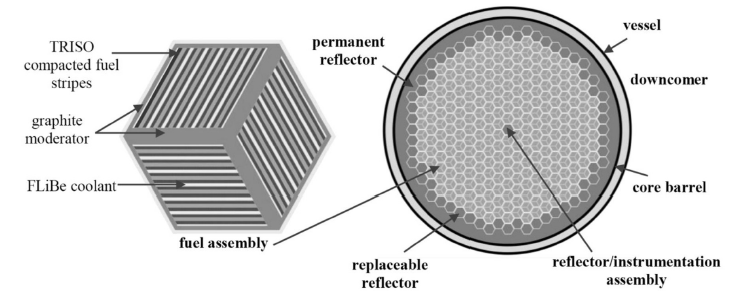
\includegraphics[width=0.9\linewidth]{ahtr.png} 
    \caption{FHR core configuration and fuel element \cite{ramey_monte_2018}.}
    \label{fig:ahtr}
\end{figure}

\subsection{Previous AHTR modeling efforts and challenges}
Modeling and simulation of the \gls{AHTR} design has been an ongoing effort 
since its conception in 2003 \cite{forsberg_molten-salt-cooled_2003}. 
The \gls{AHTR} core design differs significantly from the present \gls{LWR}-based 
nuclear power plants. 
These differences lead to modeling challenges and the need for verification and 
validation of modeling and simulation methods \cite{ramey_monte_2018}. 
Verification and validation of neutronics and thermal hydraulics tools' 
capability to successfully model the \gls{AHTR} design is a crucial step 
in support of licensure of the \gls{AHTR} design towards the eventual goal 
of deployment \cite{rahnema_phenomena_2019,rahnema_current_2015}. 
Several neutronic studies have been completed along the way to the current 
\gls{AHTR} design \cite{ramey_monte_2018,holcomb_fluoride_2013,greene_pre-conceptual_2010}. 
These efforts have shed light on the technical challenges facing the \gls{AHTR} design. 

In an effort to understand the challenges of \gls{FHR} materials, 
modeling the neutronics and thermal hydraulics in 
both plate and pebble fuelled \glspl{FHR}, a university-led Integrated 
Research Project \cite{zhang_integrated_2019} was conducted. 
During the research project, a panel of subject matter experts came together to 
generate a \gls{PIRT} by identifying phenomena and ranking their importance.
The \gls{PIRT} identifies areas in which additional research is needed to better 
understand important phenomena for adequate future modelling 
\cite{rahnema_phenomena_2019}. 
The phenomena identified as requiring further research are included in 
Table \ref{tab:phenomena}. 

\begin{table}[]
    \centering
    \onehalfspacing
    \caption{\gls{FHR} physical phenomena requiring further research 
    \cite{rahnema_phenomena_2019}.}
	\label{tab:phenomena}
    \small
    \begin{tabular}{l|l}
    \hline
    \textbf{Category} & \textbf{Phenomena} \\ \hline
    Fundamental cross section data & - Moderation in FliBe \\
    & - Thermalization in FliBe \\
    & - Absorption in FliBe \\
    & - Thermalization in carbon \\
    & - Absorption in carbon \\ \hline
    Material Composition & - Fuel particle distribution \\ \hline
    Computational Methodology & - Solution Convergence \\ 
    & - Granularity of depletion regions \\
    & - Multiple heterogeneity treatment for generating multi-group \\ 
    & cross sections \\
    & - Selection of multi-group structure \\
    & - Boundary conditions for multi-group cross section generation \\ \hline 
    General Depletion & Spectral history \\ \hline 
    \end{tabular}
    \end{table}

The \gls{AHTR} has a complex core design due to the multiple heterogeneity present 
in the fuel introduced by presence of \gls{TRISO} particles embedded in plates 
\cite{ramey_monte_2018,rahnema_phenomena_2019}.
Accurately modeling the \gls{FHR}'s complex geometry with individual \gls{TRISO}
particle fidelity is necessary to obtain detailed reference power distributions 
to assess the accuracy of lower-fidelity models.
However, it is challenging, particularly for deterministic codes which 
use multigroup cross sections and traditional homogenization methods
\cite{ramey_monte_2018}. 
These traditional homogenization methods are insufficient to capture the correct physics 
in \glspl{FHR}, due to the multiple heterogeneity \cite{ramey_monte_2018}. 
In the \gls{AHTR}, single and multiple slab homogenization decreased computation time 
by 10, however they introduce a nontrivial error of $\sim$3\%
\cite{ramey_monte_2018,cisneros_neutronics_2012}.
Core physics parameters with acceptable uncertainty must be calculated to determine 
the feasibility and safety of the \gls{AHTR} design.
For Monte Carlo codes, statistical uncertainties must be reduced by increasing 
the number of neutron histories, however this comes at an increased 
computational cost.

Another technical challenge faced by the \gls{AHTR} design is the uncertainty of 
the graphite and carbonaceous moderator material properties: densities, temperatures
and thermal scattering data.
Also, the thermal scattering data ($S(\alpha,\beta)$ matrices) for the bound 
nuclei in the \gls{FLiBe} salt are lacking \cite{ramey_monte_2018}. 
Upon examination of the thermal scattering behavior of solid \gls{FLiBe}
\cite{mei_investigation_2013} and liquid \gls{FLiBe} \cite{zhu_thermal_2017}, 
it was observed that the bound and free atom cross section of \gls{FLiBe} are 
identical above 0.1eV and diverges below 0.01eV. 
This means that the use or absence of thermal scattering data will impact the 
accuracy of the results \cite{ramey_monte_2018}. 

\subsection{AHTR Benchmark}


\section{Artificial Intelligence Applications to Nuclear Reactor Design}
